\documentclass[12pt]{article}

\usepackage{graphicx}
\usepackage{cleveref}
\begin{document}

\subsection{Ref Commentary:}
 This paper provides an elegant solution to a novel problem -- I like it a great
 deal. Most of the comments below are cosmetic suggestions for the benefit of a
 reader who has not previously thought about the problem, although there are one
 or two occasions where I think that a more comprehensive experiment is
 warranted.
 
\subsection{two related larger concerns about clarity in the whole
procedure}

1. The authors objective is the MI between one observed hitting time and
the corresponding posterior (this is only briefly mentioned in passing
above equation (8).) How is this stimulus then employed in practice --
do we start it over again after each hitting time? Is it intended to
cover the entire experiment? I think the authors do the former, but they
have never explicitly said so and I have had to infer this indirectly.
The initial discussion covers a sequence of hitting times to be treated
as data and the transition is not made clear.

The "reset the stimulus each time" approach makes sense; you get to treat each
hitting time as i.i.d. However, it's not clear that the optimal sequence of
stimuli over hitting times is the same as repeating the optimal stimulus each
time -- even without an update on the prior. I could be incorrect in this,
though, and anything the authors can say about this would be useful.


$>>$ Absolutely. Even and especially in the batch context a sequence of
different controls may result in better estimators. However, it is not clear how
to select this sequence, i.e.\ there is no natural extension to our formalism
that would spit out a sequence of controls. A lesser, practical issue is that
when computing the estimates using Max-likelihood it is simpler to have one
control than a sequence (you have to solve less PDEs). 
We have clarified this in the new section 2.2 (see next question)


2. The batch versus sequential design framework also comes as a surprise
and is not discussed at all until Section 5. The approach of updating
the prior to obtain new controls is natural, but we shouldn't have to
find out about it half way through the paper; we can also ask whether it
is optimal for the sequence of experiments. (Section 6.1 is also left
hanging, I'll come back to that later).

It really would be useful for the authors to specify the imagined experiment in
the introduction and discuss some of the considerations above. That would have
saved this reader, at least, some considerable confusion.

$>>$ Very good point on describing the 'experiment' in the introduction (in a
separate sub-section, clearly delineated). We do this and address
this and the former comments in the end subsection of Sec 2. ('Experiment
Description')

\subsection{More localized comments} 

1. Page 4; it would be helpful to move the definition of U(x,t) closer to
equation (6). It's currently given as an after-thought three paragraphs above,
making it difficult to find.

$>>$ Ok, move defn of U just prior to eq 6

2. Page 6 equation 12; it would be helpful to write out $p_{\theta}(x,t)$ to
make clear that $p_{\theta}$ is neither a constant nor a function that takes the
term in brackets as its argument.

$>>$ add arguments to $p,f,\phi$ on eq 11 (and make it all one eq instead of
two 11 and 12 per line)

3. Page 8, the expression on first term on the second line of (13) has been
half-simplified. The authors have included the multiplier and the numerator of
the logarithm that they differentiate, but they have cancelled the denominator.
Why not just simplify the whole way?

$>>$ sure, we simplify all the way, although it always takes us a few seconds of
staring at this expression to see why it's true. 

4. Page 8, following "Note that" -- it might be useful to briefly indicate that
this follows from interchanging the order of integration with respect to
$\theta$.

$>>$  good point. 

5. End of Page 8; it would be helpful to collect these results to give an
equation for calculating $\delta I$. This might also be a good point at which to
discuss the computational complexity of the estimate -- given that the authors
do appear to run into computational limits, the need to discuss computing
somewhere.

$>>$ We are a little at a loss with this comment because $\delta I$ is given as
a formula in eq (14 in the resubmited draft) and its computational steps are
outlined in sec. 3.2 immediately following it. The computational scheme for
$p,f$ (Crank-Nicholson) is referred to in Section 4, but this is such a common
technique for numerical pde's that we thought there are much better explanations in the
references (e.g Numerical Recipes for C) then we can provide - the PDEs are
linear so there really are no issues apart from standard numerical PDEs issues. 

6. Figure 1; can the authors show the threshholding at -2?

$>>$ Done.

7. Section 4.2, Figure 3 I'm assuming that the authors have represented
$\alpha(t)$ here as a step function (switching type?) for the purposes of
exploring sensitivity. A quick equation would help make that explicit.

$>>$ New equation describing the step-function form for alpha in Fig. 3 is given
in the figure caption.

7b. If this is the case, it would make sense to consider this parameterized form
for alpha(t) in their experiments. It does appear to have achieved better MI than we
see in Figure 2, for example. In suggesting this, I do not feel that the authors
more detailed work should be discounted -- we have only discovered this form because of it.

$>>$ We have now illustrated the 'optimal' objective vs. the objective values
arising from the switch-time sweep. INdeed, there are cases when the
switching-type control is marginally better than the solution to the iterative
optimization, we have commented briefly in the section 

8. Section 4.3; the authors have considered going from a 2-point prior to a 3
point prior. That seems a bit incremental. If the purpose is to show adequacy,
then a comparison with something closer to continuous -- say 10 points from
something Gaussian? I'm aware that this might be infeasible for online
estimation, but they can surely manage this once; or ought to detail why the
burden becomes high so quickly.

$>>$ We now use 11 points, the computation of a single optimization ascent
with 11 points takes on the order of 5 seconds on my laptop (dual core intel,
2.67Ghz) and computation time scales linearly with the number of points in
the prior (up to memory limitations, which depend on the refinement of the PDE
grid and time-discretization). We have indicated this at the end of section 4.1.

8b. Why, in Figure 4, are the optimal controls for both 2 and 3 point priors so
much "cleaner" than in other figures -- these look much more like the switching
functions than Figures 2 or 5.

$>>$ It turns out that we used a different initial condition for the optimizer
in these figures, we now use the same as in figs 1:5, for consistency, leaving
the question of optimization initial guess to the second last sub-subsection of
sec. 4.3. 

9. Section 5.2 appears to repeat the experimental parameters from a previous
paragraph -- the authors can save some space with this. 

$>>$ We feel that it is pedagogical to re-state those parameters again there.  

10. Page 16; the use of $N_s$ hitting times in each block makes sense if we
reset the control each time, but it was only here that I inferred that that was what
you must be doing. See my initial comments.

$>>$ Yes, indeed, each block has the same control applied $N_s$ times to obtain
one estimate using $N_s$ hitting-times. We've clarified at the beginning of
section 5.2. 

11. Figure 8 and preceding discussion suggests a likely correlation between
$\mu$ and $\tau$ -- this could be better demonstrated with a scatterplot.

$>>$ WE provide such a scatter plot along with some comments in Fig. 8 and the
end of section 5.

12. Section 6.1 does not appear particularly connected to the rest of the paper
and indeed ends mid-sentence. One doesn't need particle filters to update a
two-point prior and I wonder whether this wasn't left-over from a more
computationally-ambitious phase of the project.

$>>$ This was sloppy - actually, there are two hanging words at the end of the
last sentence, which should have been removed. (', also see'). 

We have reduced section 6.1 to a reference to the online supplemental and
previous work. As the referee mentioned all our tools used here are standard and
easily found in other references. 
\clearpage

13. Section 6.2.2 -- the obvious comparison is to performance in the batch
experiments. It would be useful to see these. It would also be useful to see the
evolution of the optimal control.
 
$>>$
It turns out that for this problem, in particular the parameter regime used to
illustrate the technique, the online-updated controls look very similar to the
ones found in the batch case, this is somewhat expected given our result in sec.
4.3 (e.g. figure 5). 
Indeed they change very little in a typical run see \cref{fig:control_iterates}
below. We have indicated this in the draft. (end of section 6.2)

However, we feel it does not add much to show the the evolution of the prior
under the batch control as it is very similar to the one under the
online-updated control. 


\begin{figure}[htp]
\begin{center}
  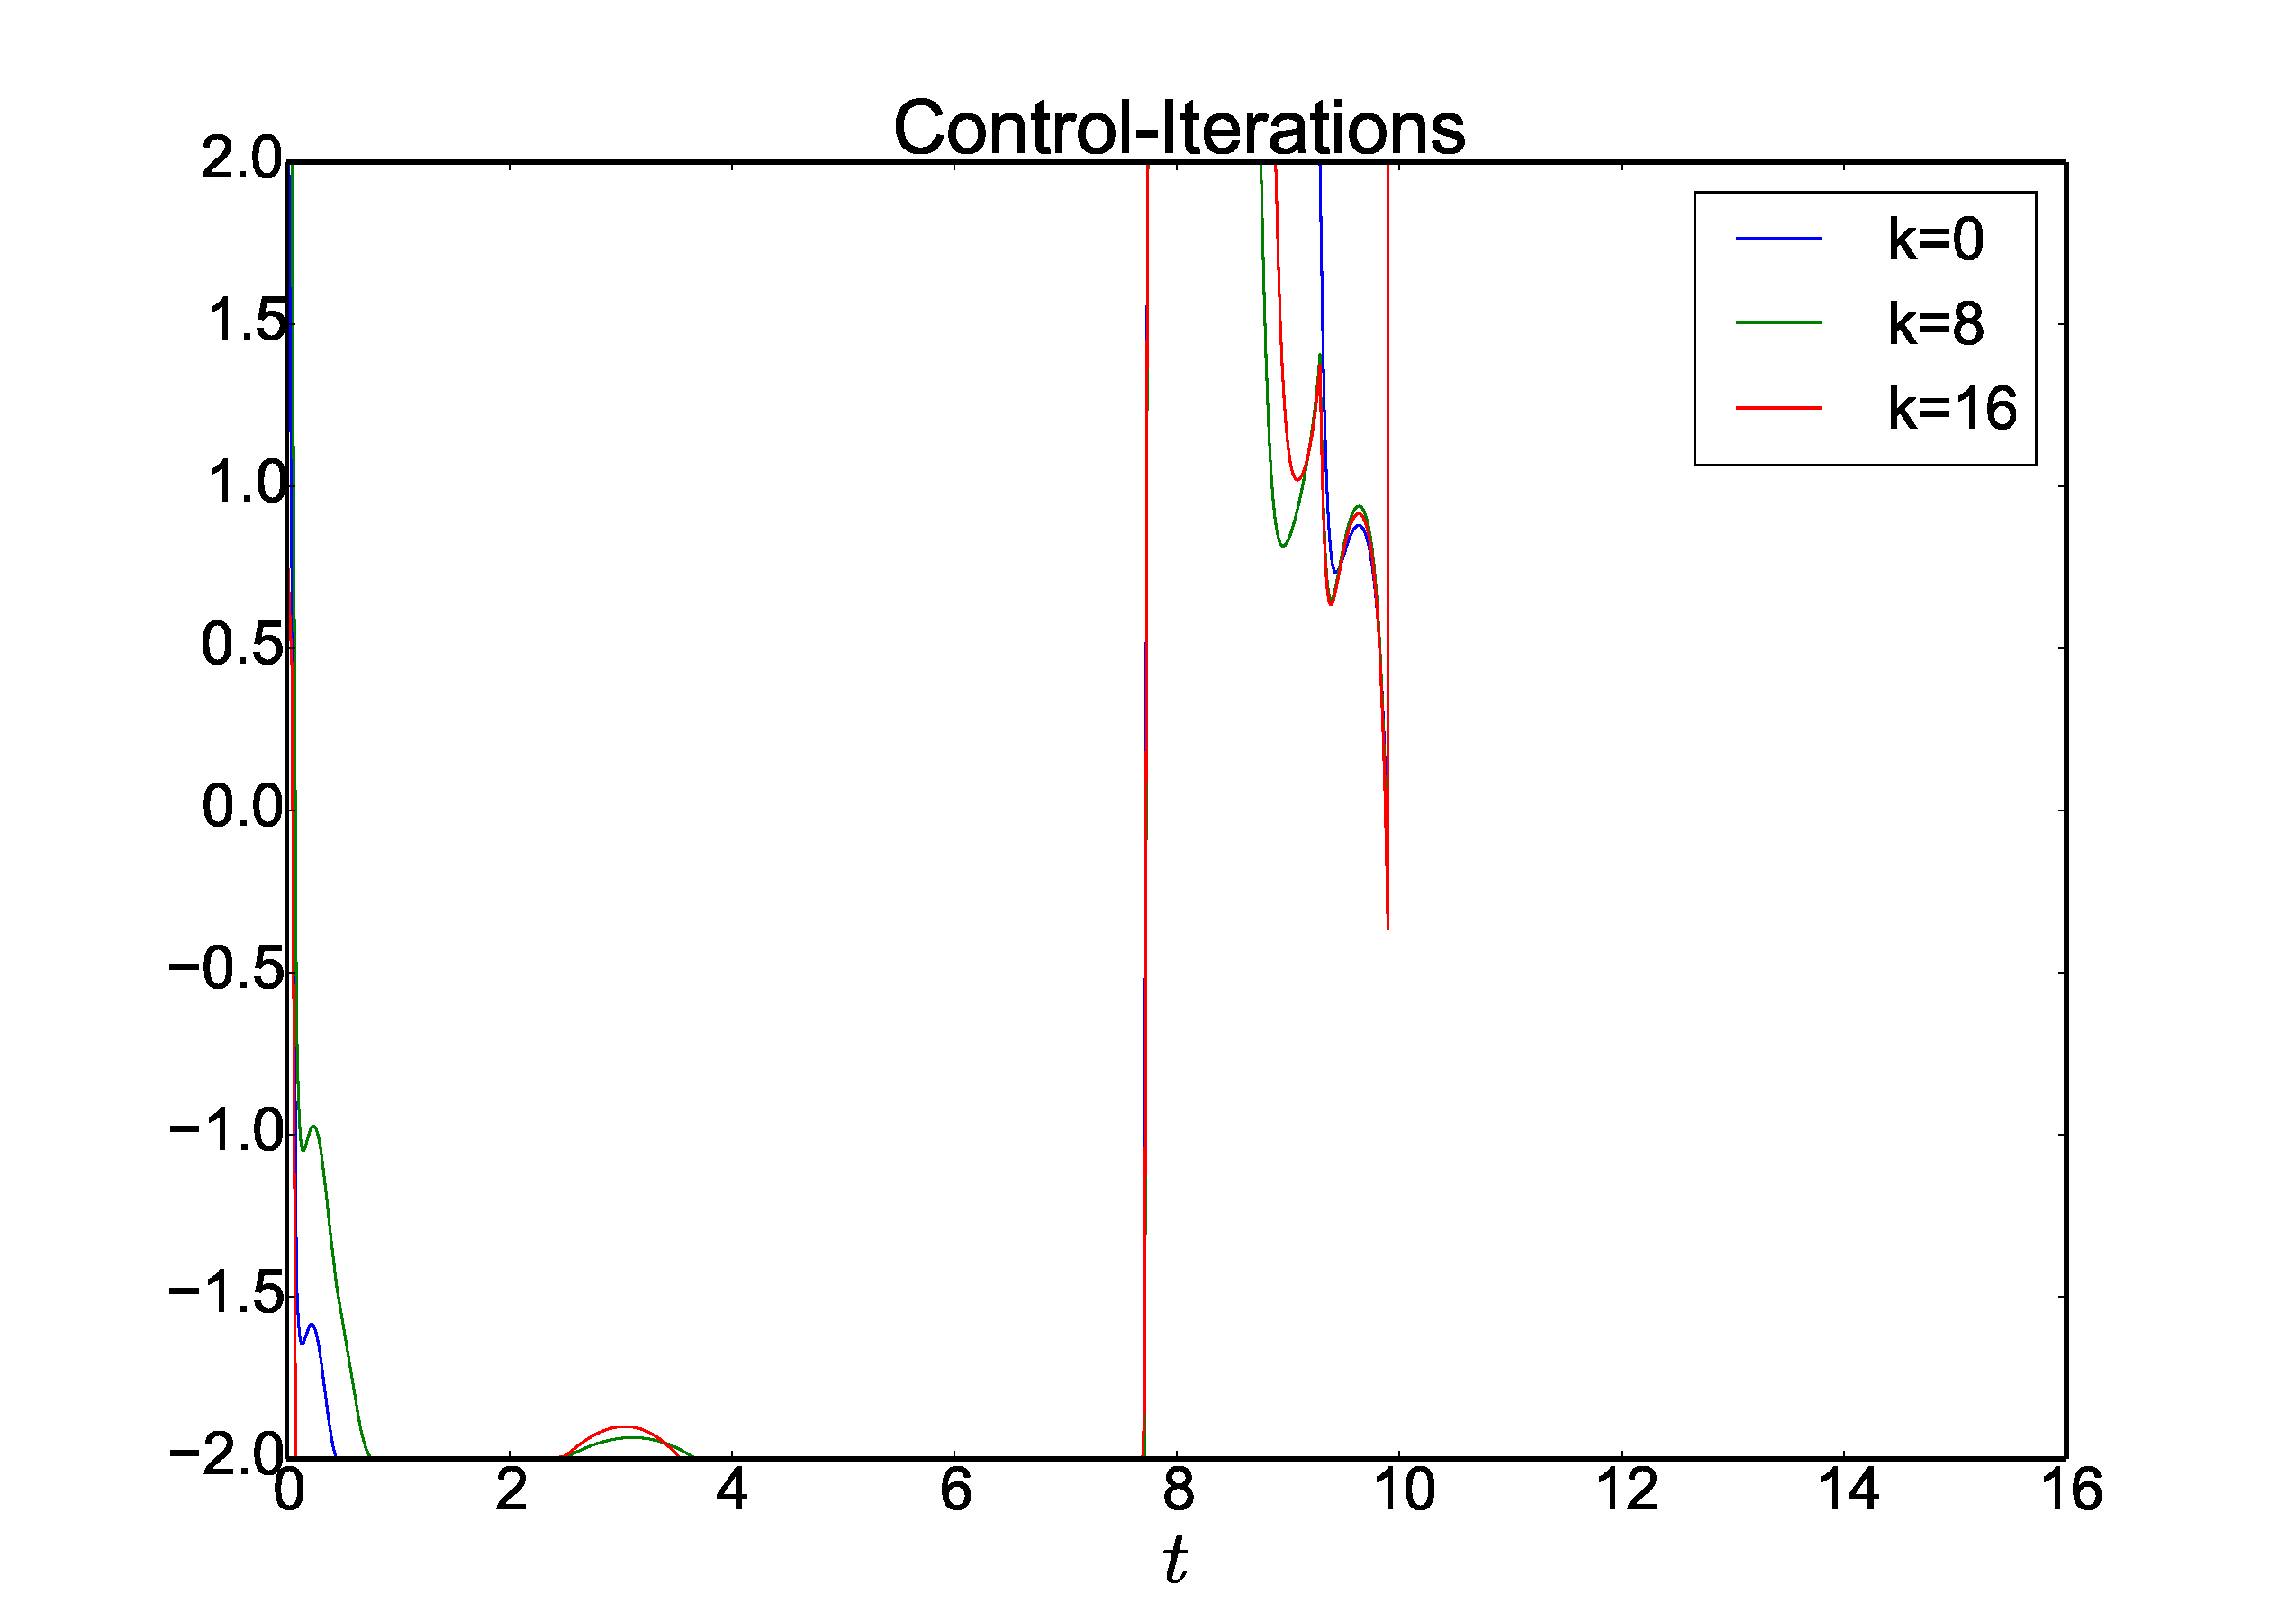
\includegraphics[width=.8\textwidth]{Figs/HTOnlineEstimator/single_experiment_example_controls_evolution.pdf}
  \caption[]{Stimulation Control changes very little throughout   online
  experiment, shown are the first 3 increments (updating after every 16
  iterations)}
  \label{fig:control_iterates}
\end{center}
\end{figure}
 
14. How generalizable is this method? It ought to work generally for linear SDEs
with observations corresponding to boundary hitting (crossing?) times. Would the
adjoint calculations break down for nonlinear systems? What if a marked point
process were observed?

$>> $In principle the formalism can be applie to any SDE, the adjoint
calculations carry essentially unperturbed for the non-linear drift/ diffusion
terms, $U(x,t), \sigma(x,t)$. So if the SDE was non-linear, then the PDEs in our
problems themselves remain linear and all calculations remain as is. The PDEs
will become non-linear if we move to more esoteric processes where $U,\sigma$
are functions of the probability density $f$ as occurs in optimal transport or
mean-field games, for example. There are also examples of this in neural
population models. We have briefly touched on this at the end of the discussion.



\end{document}